\documentclass{beamer}

\usetheme[numbering=fraction,block=fill]{metropolis}  
%\usetheme{Copenhagen} 


\usepackage{amsmath, amssymb, amsthm}
\usepackage{mathtools}
\usepackage{proof}
\usepackage{bussproofs}
\usepackage{color}
\usepackage{geometry}
\usepackage{enumerate}
\usepackage{extarrows}
\usepackage{verbatim}
\usepackage{algorithm}
\usepackage[ampersand]{easylist}
\usepackage[linewidth=1pt]{mdframed}
\usepackage[font=large,labelfont=bf]{caption}
\usepackage{float}
\usepackage{diagbox}
\usepackage{listings}

\lstdefinelanguage{snesl}
{ morekeywords={
  	def,
    else,
    function,
    if,
    in,
    let,
    then,
    T,
    F
  },
  sensitive=true, % keywords case-sensitive
  morecomment=[l]{--}, % l-line comment
  morecomment=[s]{\{-}{-\}}, % s-start and end
  otherkeywords={:,\&,\#,\%,++},
  morestring=[b]" % strings are enclosed in double quotes
}

\lstdefinestyle{snesl-style}{
	language={snesl},
	emph=[1] {concat,index,	lshift, not, ord, part,
		_plus, rshift, scatter,
	},
	emphstyle=[1]{\color{blue}}
}


\lstdefinelanguage{svcode}
{  morekeywords={
		WithCtrl,
		SCall,
	},
	sensitive=true, 
	morecomment=[l]{--}, 
	otherkeywords={:=},
}

\lstdefinestyle{svcode-style}{
	language={svcode},
	emph=[1] {:= },
	emphstyle=[1]{\color{blue}}
}


\lstset{
	basicstyle=\scriptsize\ttfamily,
	breakatwhitespace=true,
	breaklines=true,
	captionpos=t,
	columns=fixed,
	extendedchars=true,
	commentstyle=\color{darkgreen},
	frame=single,
	frameround=tttt,
	framesep=4pt,
	keywordstyle=\bfseries\color{carnelian},
%	numbers=left,
	numberstyle=\scriptsize\color{gray},
	rulecolor=\color{black},
	showstringspaces=false,
	showtabs=false,
	stepnumber=1,
}


\def\*#1{\mathbf{#1}}

%source language syntax
\def\Let#1#2#3{\*{let} \ #1 = #2 \ \*{in} \ #3}
\def\Comp#1#2#3#4{\{#1 : #2 \ \*{in} \ #3 \ \*{using} \ #4\}}
\def\RComp#1#2#3{\{ #1 \ | \ #2 \ \*{using} \ #3 \}}

\def\hcall{\phi} 

\def\usevars{x_1,...,x_j}
\def\usevarsk{x_1,...,x_k}
\def\j#1{(#1)^j_{i=1}}
\def\k#1{(#1)^k_{i=1}}
\def\l#1{(#1)^l_{i=1}}

\def\const#1{\*{const}_{#1} ()}
\def\iota#1{\*{iota} (#1)} 
\def\plus#1#2{\*{plus} (#1,#2)}

\def\constn#1{\*{const}_{#1}}
\def\iotan{\*{iota}} 
\def\plusn{\*{plus}}


%types
\def\int{\*{int}}
\def\bool{\*{bool}} 
\def\tseq#1{\{#1\}}  


% symbol shorthands
\def\Eva{\downarrow}
\def\Ra{\Rightarrow}
\def\Env{\ \vdash\ } 

\def\Seqk#1{\{ #1_1,...,#1_k \}}
\def\Tupk#1{(#1_1,...,#1_k)}
\def\replc#1#2{#2_1,...,#2_{#1}}

% greek letters
\def\sgm{\sigma}
\def\Gam{\Gamma}
\def\del{\delta}


% special font

\def\MC{\mathcal{C}}  % translation
\def\ME{\mathcal{E}}  % snesl evaluation
\def\MP{\mathcal{P}}  % svcode semantics
\def\MT{\mathcal{T}}  % typing rules
\def\MR{\mathcal{R}}  % value representation


% Judgment
\def\Jug#1{\textbf{Judgment} \boxed{#1} \\[1ex]}

\def\Map#1#2{#1 \mapsto #2}
 

% Evaluation
\def\Eval#1#2#3{#1 \Env #2 \Eva #3 } 
\def\EvalF#1#2#3{#1(#2) \Eva #3}  % function evaluation

%typing
\def\Type#1#2#3{#1 \Env #2 : #3 } 
\def\Typef#1#2#3{#1 : (#2) \rightarrow #3}
\def\TypeV#1#2{#1 : #2}

%value representation
\def\ValRep#1#2#3{ #1 \triangleright_{#2} #3}


% rule with a name
\def\ERule#1#2{$\textsc{E-#1} : {#2}$}
\def\CRule#1#2{$\textsc{C-#1} : {#2}$}
\def\PRule#1#2{$\textsc{P-#1} : {#2}$}


% only rule name
\def\EName#1{\textsc{E-#1}}
\def\PName#1{\textsc{P-#1}}
\def\CName#1{\textsc{C-#1}}

%proof tree shorthands
\def\AC#1{\AxiomC{$#1$}}
\def\Axiom#1{\AxiomC{} \UnaryInfC{$#1$}}
\def\UC#1{\UnaryInfC{$#1$}}
\def\BC#1{\BinaryInfC{$#1$}}
\def\TC#1{\TrinaryInfC{$#1$}}
\def\DP{\DisplayProof}
\def\LeLa#1{\LeftLabel{$#1$}}
\def\RiLa#1{\RightLabel{$#1$}}
\def\PT#1{#1 \DisplayProof \qquad} 
%UnaryInfC with a deriviation name
\def\UCN#1#2{\AxiomC{$#1$} \noLine \UC{#2}}


%shorhands notations
\def\<{\langle} 
\def\'>{\rangle}
\def\->{\rightarrow}
\def\=>{\Rightarrow}

\def\ConEq#1{\xlongequal{<#1}}  % Sgm conditional equation
\def\.<{\lessdot}
\def\bs{ \ \backslash \ } 

\def\olol#1{\overline{\overline{#1}}}

\def\unit{()}
\def\vunit{\langle \unit \rangle}  

\def\vrange#1#2{\langle #1,...,#2 \rangle}
\def\lrange#1#2{\left[ #1,...,#2 \right]}

\def\emptyv{\langle \rangle}

\def\prefix{\sqsubseteq}


\def\s{\mathit{s}}  
\def\st{\mathit{st}} 
\def\SId{\mathbf{SId}}
\def\STree{\mathbf{STree}}

\def\sset{\mathbb{S}}
\def\S{S}
\def\Sin{S_{in}}
\def\Sout{S_{out}}

\def\FV#1{\mathtt{fv}(#1)}
\def\dv#1{\mathtt{dv}(#1)}


\def\v{w}
\def\a{\vec a}
\def\b{\vec b}
\def\c{\vec c}

\def\SvVal{\mathbf{SvVal}}

%\def\ctrl{\mathtt{Ctrl}}
\def\consta#1{\mathtt{Const_{#1}}} 
\def\toflag{\mathtt{ToFlags}}
\def\usum{\mathtt{Usum}}
\def\maptwo#1{\mathtt{MapTwo}_{#1}}
\def\map#1{\mathtt{Map}_{#1}}

\def\scan{\mathtt{ScanPlus}}

\def\genscan{\mathtt{Scan}}
\def\genreduce{\mathtt{Reduce}}

\def\distr{\mathtt{Distr}}
\def\pack{\mathtt{Pack}}
\def\upack{\mathtt{UPack}}
\def\bu{\mathtt{B2u}}
\def\segconcat{\mathtt{SegConcat}}
\def\usegcount{\mathtt{USegCount}}
\def\intermerge{\mathtt{InterMerge}}
\def\seginter{\mathtt{SegInter}}
\def\primseginter{\mathtt{PrimSegInter}}
\def\check{\mathtt{Check}}
\def\isempty{\mathtt{IsEmpty}}
\def\emptyctrl{\mathtt{EmptyCtrl}}



\def\constaf#1{\mathtt{Const_{#1}()}} 
\def\toflagf#1{\mathtt{ToFlags}(#1)}
\def\usumf#1{\mathtt{Usum}(#1)}
\def\maptwof#1#2#3{\mathtt{MapTwo}_{#1}(#2,#3)}
\def\scanf#1#2{\mathtt{ScanPlus}(#1,#2)}
\def\distrf#1#2{\mathtt{Distr}(#1,#2)}
\def\packf#1#2{\mathtt{Pack}(#1,#2)}
\def\upackf#1#2{\mathtt{UPack}(#1,#2)}

\def\:={:=}
\def\sdef#1#2{#1 := #2}
\def\withctrl#1#2#3#4{#4 := \mathtt{WithCtrl}(#1,#3,#2)}
\def\wc{$\mathtt{WithCtrl}$ }
\def\sc{$\mathtt{SCall}$ }
\def\scall#1#2#3{#3 := \mathtt{SCall} \ #1(#2)} 
\def\sf{$\mathtt{SFun}$}

\def\T{\mathtt{T}} 
\def\F{\mathtt{F}} 
\def\oT{\singl{\T}}
\def\oF{\singl{\F}}

\def\sids#1{\mathtt{sids}(#1)}
\def\ol#1{\overline{#1}}

\def\++{+\!+}
\def\vapp#1#2{#1 {\++} #2}


\def\~#1{\stackrel{#1}{\sim}}
\def\x#1{\stackrel{#1}{\bowtie}} % sgm append

\newcommand\ra{\rightarrow}
\def\Da{\Downarrow}
\def\dda{\downdownarrows}

\def\lcall{\psi} 


\def\blockf#1#2#3{#1(#2) \Eva #3} 
\def\unary#1#2#3{{\lcall}(#1,...,#2) \dda #3}

\def\blockv#1#2#3#4{\lcall_{#1}(#2,...,#3) \Eva #4}  
\def\unaryv#1#2#3#4#5{\lcall_{#1}(#2,...,#3) \dda^{#4} #5}

\def\singl#1{\langle #1 \rangle}
\def\|->{\mapsto}   % map 
\def\>->{\rightarrowtail} % map a bunch of variables
%\def\=>#1#2{\Rightarrow^{#1}_{#2}}


%translation
\def\sfun#1#2{(#1,#2)}

% compiling/translation
\def\Trans#1#2#3#4#5{#1 \Env #2 \Rightarrow^{#3}_{#4} #5}
\def\Transf#1#2#3#4#5{#1(#2) \Rightarrow^{#3}_{#4} #5}

%% ---- formalization
\def\Vtransb#1#2#3#4{#1 \mathrel{\triangleleft_{#2}} #3,#4}
\def\wf#1#2#3{ #2 \Vdash #1 : #3} %well-formed
\def\etail#1#2{\< #1 | #2 \'>}  % element and a tail vector

\def\PRName#1{\textsc{I-#1}}
\def\MI{\mathcal{I}}  % prefix rule
% well-formedness rules
\def\WName#1{\textsc{W-#1}}
\def\MW{\mathcal{W}}

\def\ConEq#1{\xlongequal{#1}}  % Sgm conditional equation

\def\Seql#1{\{ #1_1,...,#1_l \}}
\def\emptyvtau#1{\emptyv_{#1}} 



\newtheorem{thm}{Theorem}
\newtheorem{lem}[thm]{Lemma}
\newtheorem{defi}[thm]{Definition}
\newtheorem{nota}[thm]{Notation}
\newtheorem{prop}[thm]{Proposition}
\newtheorem{cor}[thm]{Corollary}

        
\title{Formalizing the implementation of \\ Streaming NESL}
\subtitle{Master's Thesis}

\author{Dandan Xue}
\date{Novermber 8, 2017}

\institute{Department of Computer Science (DIKU) \\ University of Copenhagen}

\begin{document}
\maketitle

\begin{frame}{Contents}
\setbeamertemplate{section in toc}[sections numbered]
\tableofcontents[hideallsubsections]
\end{frame}


\section{Introduction}

\begin{frame}{NESL}

	\begin{itemize}
		\item A functional nested data-parallel language
		\item Developed by Guy Blelloch in 1990s at CMU
		\item Highlights: 
		\begin{itemize}
			\item Highly expressive for parallel algorithms. \\ 
			\begin{itemize}
			
			\item Data-parallel construct: \emph{apply-to-each} $$\{e_1(x) : x \ \*{in} \ e_0 \} $$\\ 
	  \item Ex: compute $\sum_{i=1}^{2}i^2$ and $\sum_{i=3}^{10}i^2$:
	  $$\{\*{sum}(\{i \times i: i \ \*{in} \ s\}) : s \ \*{in} \ [[1,2],[3,4,5,6,7,8,9,10]]\}$$
	  ! Allocate {\color{blue} 10} size of space for intermediate data
  		\end{itemize}
	  \item An intuitive cost model for time complexity: work--step model
	  \begin{itemize}
	  	\item work cost $t_1$: total number of operations executed
	  	\item step cost $t_\infty$: the longest chain of sequential dependency
	  \end{itemize}
	\end{itemize}
	\end{itemize}
  
\end{frame}

\begin{frame}{Streaming NESL (SNESL)}
	\begin{itemize}
		\item Experimental refinement of NESL
		\item Aiming at improving space-usage efficiency 
		\item Work by Frederik Madsen and Andrzej Filinski in 2010s at DIKU
		\item Highlights:
		\begin{itemize}
			\item Streaming semantics 
			\begin{align*} 
			& \pi ::= \bool \ | \ \int \ | \ \*{char} \ | \ \*{real}  \ | \ \cdots \tag{scalar types}\\
			& \tau ::= \pi \ | \ (\tau_1,...,\tau_k) \ | \ [\tau] \tag{concrete types} \\
			& \sigma ::= \tau \ | \ (\sigma_1,...,\sigma_k) \ | \ \tseq{\sigma}  \tag{streamable types} 
			\end{align*}
			
			\item A space cost model
			\begin{itemize}
				\item sequential space $s_1$: the minimal space to perform the computation
				\item parallel space $s_\infty$: space needed to achieve the maximal parallel degree (NESL's case)
			\end{itemize}
		\end{itemize}
	\end{itemize}
\end{frame}

\begin{frame}{SNESL syntax} \small
	\begin{itemize}
		\item<1-> Expressions
		\begin{alignat*}{2}
		& e &&::=  a \ | \ x \ | \ (e_1,...,e_k) \ | \ \Let{x}{e_1}{e_2} \ | \ \hcall{\Tupk{e}} \\ 
		&   && \quad | \ \{e_1:  x \ \*{in} \ e_0 \} \tag{general comprehension} \\
		&   && \quad | \ \{e_1 \ | \ e_0 \}\tag {restricted comprehension} 
		\end{alignat*}	
  \item<2-> Primitive functions
		\begin{alignat*}{2} 
		&\hcall && ::= \oplus \ | \ \ \*{append} \ | \ \*{concat} \ | \ \*{zip} \ | \ \*{iota}  \ | \ \*{part}  \ | \ \*{scan}_{\otimes} \ | \ \*{reduce}_{\otimes}   \\
		&   && \quad | \ \*{mkseq} \ |  \ \*{the}  \ | \ \*{empty} \tag{sequence operations}\\
		&   && \quad | \ \*{length} \ | \ \*{elt}  \tag{vector operations}\\
		&   && \quad | \ \*{seq} \ | \ \*{tab} \tag{convertion between vector and sequence}\\
		& \oplus  \ && :: = +  \ | \ \times \ |  \  / \ | ==  \ | \ \*{not} \ | \ \cdots  \tag{scalar operations}\\
		& \otimes \ && :: = + \ | \ \times  \ | \ \*{max} \ | \ \cdots  \tag{associative binary operations}
		\end{alignat*} 
\item<3-> $\*{if} \ e_0 \ \*{then} \ e_1 \ \*{else} \ e_2 \equiv \Let{b}{e_0}{ \*{the}(\{e_1 \ | \ b \} {\++} \{e_2 \ | \ \*{not}(b)\})} $

	\end{itemize}
\end{frame}

\begin{frame}[fragile]{SNESL primitive functions}
	\begin{table}\footnotesize 
		\begin{tabular}{p{0.35\columnwidth}|p{0.63\columnwidth}}
			\hline
			$\*{append : (\{\sgm\}, \{\sgm\}) \ra \{\sgm\}}$ &  syntactic sugar ${\++}$; $\{3,1\} {\++} \{4\} = \{3,1,4\}$ \\ \hline
			$\*{concat: \{\{\sgm\}\} \rightarrow \{\sgm\} }$ &  $\*{concat}(\{\{3,1\},\{4\}\}) = \{3,1,4\}$                \\ \hline
			$\*{zip} \colon (\{\sgm_1\}, ..., \{\sgm_k\})\ra \{(\sgm_1,...,\sgm_k)\}$ & $\*{zip}(\{1,2\},\{\F,\T\}) = \{(1,\F),(2,\T)\}$\\ \hline
			$\*{iota(\&): \int \ra \{\int\}}$  &  \&5 = \{0,1,2,3,4\} \\ \hline
			$\*{part: (\{\sgm\}, \{\bool\}) \ra  \{\{\sgm\}\}}$   & $\*{part}(\{3,1,4\}, \{\F,\F,\T,\F,\T,\T\}) = \{\{3,1\},\{4\},\{\}\}$                \\ \hline
			$\*{scan_\otimes}: \{\int\} \ra \{\int\}$     & $\*{scan_+}(\&5) = \{0,0,1,3,6\} $  \\ \hline
			$\*{reduce_\otimes: \{\int\} \ra \int }$     &  $\*{reduce_+}(\&5) = 10$              \\ \hline
			$\*{mkseq}: (\overbrace{\sgm,...,\sgm}^{k}) \ra \{\sgm\}$  & $\*{mkseq}(1,2,3) = \{1,2,3\}$ \\ \hline  
			$\*{length(\#)}$: $[\tau] \ra \int$ & \#[10,20] = 2\\ \hline  
			$\*{elt(!)}$: ($[\tau], \int) \ra \tau$  & [3,8,2] ! 1 = 8 \\ \hline  
			$\*{the:  \{\sgm\} \ra \sgm}$     &  return the element of a singleton,  $\*{the}(\{10\}) = 10$        \\ \hline
			$\*{empty:  \{\sgm\} \ra \bool}$       & $\*{empty}(\{1,2\}) = \F, \*{empty}(\&0)= \T$      \\ \hline  
			$\*{seq}: [\tau] \ra \{\tau\} $  & $\*{seq}([1,2]) = \{1,2\}$ \\ \hline  
			$\*{tab}: \{\tau\} \ra [\tau] $  & $\*{tab}(\{1,2\}) = [1,2]$\\ \hline  
		\end{tabular}
	\end{table}
	
\end{frame}

\begin{frame}[fragile]{SNESL example: word count} \small
%
%\lstinputlisting[style=nesl-style]{code/wordpart.nesl} 
\lstinputlisting[style=nesl-style]{code/wordpart.snesl} 
%	
\begin{lstlisting}[style=nesl-style] 
  $> slength(str2wds_snesl(read_file(filename)))
\end{lstlisting}
\pause
\begin{itemize}
	\item Takes constant space 
	\item Speedups of a similar word count program from [MF16]:

	\centering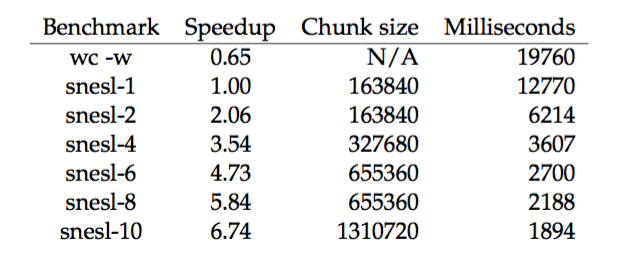
\includegraphics[width=0.6\linewidth]{tab-workcount}
		
\end{itemize}

\end{frame}


% ---------------- implemenation ------------------------------

\newcommand\tr{\triangleright}
\newcommand{\proc}{\*{Proc}}
\newcommand{\bufst}{\*{BufState}}
%\newcommand{\sups}{\*{Sups}}
\newcommand{\clis}{\*{Clis}}
\newcommand{\xducer}{\*{Xducer}}
\newcommand{\filling}{\texttt{Filling} \ }
\newcommand{\draining}{\texttt{Draining} \ }
\newcommand{\pin}{ \texttt{Pin} \ }
\newcommand{\pout}{\texttt{Pout}}
\newcommand{\done}{\texttt{Done}}
\newcommand{\ftype}{\varphi}


\def\interT#1#2#3{\vdash_{#1} #2 : #3}
\def\conc#1{#1 \ {\mathbf{concrete}}}
\def\Type#1#2#3{#1 \vdash_{\Sigma} \ #2 : #3 } 
\def\Eval#1#2#3{#1 \vdash_{\Phi} #2 \Eva #3 } 
\def\Distr#1#2#3{\mathtt{distr}_{#3}(#1,#2)}
\def\Pack#1#2#3{\mathtt{pack}_{#3}(#1,#2)}

\section{Implementation}

\begin{frame}{Source language}

\begin{itemize}
\item Simplified SNESL types
	{\small\begin{align*} 
	& \pi ::= \bool \ | \ \int  \tag{only two scalar types}\\ 
	& \tau ::= \pi \ | \ (\tau_1,\tau_2) \ | \ \tseq{\tau} \tag{no vectors, change tuples to pairs} \\
	& \ftype :: = (\tau_1,...,\tau_k) \ra \tau  \tag{support recursion}
	\end{align*}}	
\pause
\item Syntax
	{\small \begin{alignat*}{2} 
%	& t &&::= \*{eval} \ e \ | \ d \ t \  \tag{top-level term} \\
	& e &&::= \cdots | \ f (e_1,...,e_k)  \tag {user-defined function call} \\
	& d &&::= \*{function} \  f (x_1\colon{\tau_1}, ..., x_k\colon\tau_k)\colon{\tau} = e \\
%	&\hcall && ::= \oplus \ | \  \ \*{append}_{\tau} \ | \ \*{concat}_{\tau}  \ | \ \&  \ | \ \*{part}_{\tau}  \ | \ \*{scan}_+ \ | \ \*{reduce}_{+} \ | \cdots \\	
	\end{alignat*}
   }
%& \oplus  \ && :: = + \ | \ - \ | \ \times \ |  \  / \ | \ \% \ | <= \ | \ == \ | \  \*{not} \ | \ \cdots
\end{itemize}
\end{frame}

\begin{frame}{Source language}
\begin{itemize}
	\item Key typing rules, \boxed{\Type{\Gam}{e}{\tau}}: \\[2ex]
{\footnotesize
\makebox[1.2\textheight]{	
	\PT{
		\AC{\Type{\Gam}{e_0}{\{\tau_0\}}}
		\AC{\Type{[x \|-> \tau_0, \k{x_i \|-> \tau_i}]}{e_1}{\tau}}
		\RiLa{\left(
			\begin{aligned}
				&\k{\Gam(x_i) = \tau_i, \\
					&\conc{\tau_i}}
			\end{aligned} \right)}
		\BC{\Type{\Gam}{\Comp{e_1}{x}{e_0}{\usevarsk}}{\tseq{\tau}}}
	}
}\\[2ex]

%\PT{
%	\AC{\Type{\Gam}{e_0}{\bool}}
%	\AC{\Type{[\k{x_i \|-> \tau_i}]}{e_1}{\tau}}
%	\RiLa{(\k{\Gam(x_i) = \tau_i})}
%	\BC{\Type{\Gam}{\RComp{e_1}{e_0}{\usevarsk}}{\tseq{\tau}}}
%}\\[2ex]
}
%\PT{
%	\AC{\Type{\Gam}{e_1}{\tau_1}}
%	\AC{\cdots}
%	\AC{\Type{\Gam}{e_k}{\tau_k}}
%	\RiLa{(\Sigma(f) = (\tau_1, ... , \tau_k) \ra \tau)}
%	\TC{\Type{\Gam}{f(e_1,...,e_k)}{\tau}}
%}\\[2ex]
%%TODO fix or remove

\item Key evaluation rules, \boxed{\Eval{\rho}{e}{v}} : \\[2ex]

\PT{
	\AC{\Eval{\rho}{e_0}{\{v_1,...,v_l\}}}
	\AC{(\Eval{[x \|-> {v_i}, (x_j \|-> \rho(x_j))^k_{j=1}]}{e_1}{v_i'})^l_{i=1}}
	\BC{\Eval{\rho}{\Comp{e_1}{x}{e_0}{\usevarsk}}{\{\replc{l}{v'}}\}}
}\\[2ex]


%\PT{
%	\AC{\k{\Eval{\rho}{e_i}{v_i}}}
%	\AC{\Eval{[\k{x_i \|-> v_i}]}{e_0}{v}}
%	\BC{\Eval{\rho}{f{\Tupk{e}}}{v}}
%}\\
%where $\Phi(f)=   f(x_1\colon\tau_1, ..., x_k\colon\tau_k)\colon \tau = e_0$

\end{itemize}
\end{frame}

\begin{frame}{Target language: SVCODE}
	\begin{itemize}
	\item SVCODE values:
		\begin{itemize}
			\item primitive stream: $\a ::= \<a_1,...,a_l\'>$ \\ 
			e.g., $\a_1 = \<1,2\'>,  \<0 | \a_1 \'> = \<0,1,2\'>$, $\b = \<\F, \T , \F\'>$
			\item stream tree: $w ::= \a \ | \ (w_1,w_2)$
		\end{itemize}
\pause		
	\item SVCODE syntax:
		{\footnotesize \begin{alignat*}{2} 
		&p  && :: = \ \epsilon \ | \ p_1;p_2 \\ 
		&   && \quad | \ \sdef{\s}{\psi(s_1,...,s_k)}  \tag{single stream definition}\\
		&   && \quad | \ \withctrl{\s}{p_1}{\Sin}{\Sout}  \tag{\wc block}\\
		&   && \quad | \ \scall{f}{s_1,...,s_k}{(s_1',...,s_{k'}')} \tag{ function call}\\
		& \psi \ && ::= \consta{a} \ | \ \toflag  
		\ | \ \usum \ | \ \map{\oplus} \ | \ \genscan_{+} \ | \ \genreduce_{+} \ | \ \distr    \\
		&   && \quad  | \ \pack \ | \ \upack \ | \ \bu \ | \ \segconcat \ | \intermerge \ | \ \cdots  \tag{Xducers} \\
		&\s && ::= 0 \ | \ 1 \ | \ \cdots \in \SId  = \mathbb{N}   \tag{stream ids}\\
		&  \S && ::= \{\s_1,..., \s_k\} \in \sset  \tag{set of stream ids}\\	
		\end{alignat*}}
		
		\item semantics
	\end{itemize}
\end{frame}


\begin{frame}[fragile]{SVCODE dataflow DAG}
\begin{columns}
\begin{column}{0.36\textwidth}

\begin{lstlisting}[style=svcode-style]
S1 := Const_3
S2 := ToFlags S1
S3 := Usum S2
[S4] := WithCtrl S3 []:
   S4 := Const_1
S5 := ScanPlus S2 S4
\end{lstlisting}	
	\end{column}	
	\begin{column}{0.64\textwidth}
	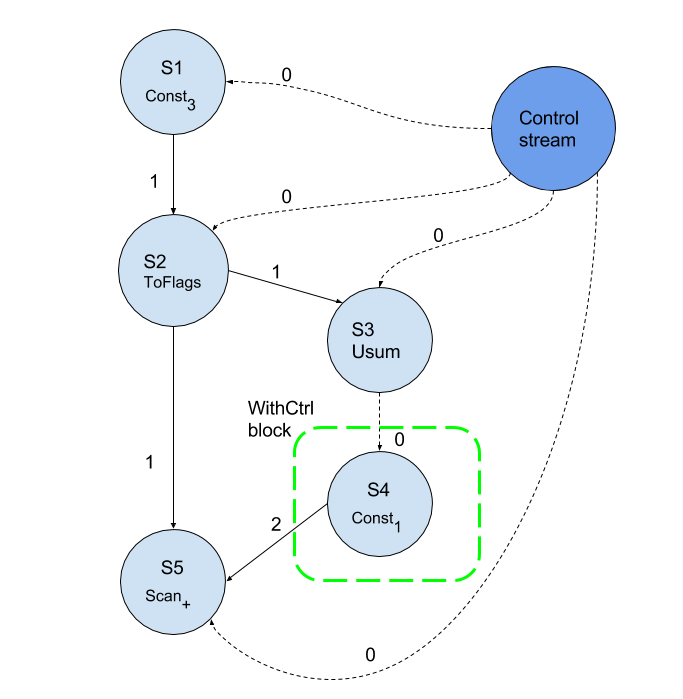
\includegraphics[width=1.1\textwidth]{../fig/dataflow.png}
	\end{column}
\end{columns}
\end{frame}


\begin{frame}{Value representation}
\begin{itemize}
%	\item Scalars are represented as singleton primitive streams: e.g., $3 \tr_\int \ \< 3 \'>, \T \tr_\bool \oT $
%	
	\item A nested sequence with a nesting depth $d$ is represented as a flattened data stream and $d$ segment descriptor streams. 
	$$\{3,1,4\} \tr_{\{\int\}} (\< 3,1,4 \'>, \< \F, \F,\F , \T \'>) $$
	$$\{\{3,1\}, \{4\}\} \tr_{\{\{\int\}\}} ((\< 3,1,4 \'>, \<\F,\F,\T,\F,\T \'>),\< \F, \F, \T \'>)  $$
	
%\item A pair of SNESL values is represented as a pair of stream trees.  
%	$$(\{\T,\F\},2) \tr_{(\{\bool\},\int)} ((\< \T, \F \'>, \< \F,\F,\T \'>),\singl{2})$$

%\item A sequence of pairs is represented as a pair of sequences sharing one descriptor:
%	$$\{(1,\T),(2,\F),(3,\F)\} \tr_{\{(\int,\bool)\}} ((\<1,2,3\'>, \<\T,\F, \F\'>), \< \F,\F,\F,\T \'>)$$
\end{itemize}
\end{frame}


\begin{frame}[fragile]{Translation}
\begin{itemize}
	\item $\STree \ni \st ::= \s \ | \ (\st_1,\st_2) $
	\item Translation symbol table $\del ::= [x_1 \|-> \st_1,..., x_k \|-> {\st_k}] $
	\item General comprehension translation:\\
	$\Comp{i+x}{i}{\&3}{x} \Ra$  
{\footnotesize
	\begin{lstlisting}[style=svcode-style]
  S4 := ...   -- <10 >    x
  S5 := ...   -- <F,F,F,T> descriptor of &3 
  S6 := ...   -- <0,1,2>  i
  S7 := Usum S5;  -- 1. generate new control:   <() () ()>
  S8 := Distr S4 S5; -- 2. replicate x 3 times: <10 10 10>
  [S9] := WithCtrl S7 [S6,S8]: -- 3. translate  (i+x)
            S9 := Map_+ S6 S8  -- <10,11,12>
\end{lstlisting}
}
%	\item Restricted comprehension translation: $\pack$ free variables instead of $\distr$
\end{itemize}
\end{frame}


\begin{frame}{Translation continued}
	\begin{itemize}
		 \item Built-in function translation: 
		\begin{itemize}
			\item $\*{scan}, \*{reduce}, \*{concat}, \*{part}, \*{empty}$: translated to a single stream definition, e.g., 
			${\*{scan}_+}{((s_d,s_b))} \Ra {\genscan_{+}(s_b,s_d)}$
			\item $\*{the}$, $\*{iota}$ translated to a few lines of code, e.g.,
			$\iota{\s} \Ra \left(
			 \begin{aligned}
			 & \sdef{\s_0}{\toflag(\s)} ; \\ 
			 & \sdef{\s_1}{\usum(s_0)} ; \\
			 & \withctrl{\s_1}{\sdef{\s_2}{\consta{1}()}}{\emptyset}{\{\s_2\}}; \\
			 & \sdef{\s_3}{\genscan_{+}(\s_0,s_2)}
			 \end{aligned} 
			 \right)$
			 
			\item $\*{++}_{\tau}$: translated recursively, depending on $\tau$
\pause
		\end{itemize}
		\item User-defined functions: translated to SVCODE functions, unfolded at runtime when interpreting a \sc 
	\end{itemize}
\end{frame}

\begin{frame}{SVCODE interpreters}
\begin{itemize}
	\item Eager interpreter (NESL-like) 
	\begin{itemize}
		\item assumes sufficient memory for allocating all streams at once
		\item executes each instruction sequentially 
	\end{itemize}
	\item Streaming interpreter
	\begin{itemize}
		\item limited buffer size, space-usage efficient
		\item result is collected from  each scheduling round
		\item DAG dynamically completed
		\item need effective scheduling strategy to avoid deadlock and guarantee cost preservation
	\end{itemize} 
	
	\item Both instrumented with cost metrics (work, step), compared with the high-level one 
\end{itemize}
\end{frame}


%\begin{frame}{SVCODE streaming interpreter}
%	\begin{itemize}
%	\item Dataflow graph is similar to a Kahn process network
%	\begin{itemize}
%		\item Graph node (a process): $\proc   =  (\bufst, \S, \clis, \xducer)$
%		\item Buffer state maintained by process: $\bufst ::= \filling \ \a  \ | \ \draining \ \a \ b$ 
%		\item A process example: 
%	\end{itemize}
%
%	\end{itemize}
%	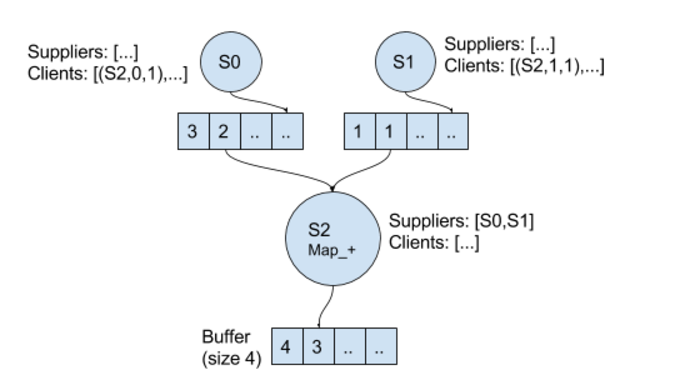
\includegraphics[width=0.8\textwidth]{../fig/process}
%\end{frame}


\begin{frame}[fragile]{Recursion example}
A function to compute factorial:
\begin{lstlisting}[style=nesl-style]
> function fact(x:int):int = if x <= 1 then 1 else x*fact(x-1)
> let s = {3,7,0,4} in {fact(n): n in s}
\end{lstlisting}
\pause
1st unfolding (will unfold 7 times in total):
\lstinputlisting[style=svcode-style]{code/fact.svcode}	
    
\end{frame}


% ---------------- Formalization ------------------------------
\def\fmsnesl{SNESL\textsubscript{0}}
\def\fmsvcode{SVCODE\textsubscript{0}}

\def\seval#1#2#3#4#5{\left\langle#1,#2 \right\rangle \Da^{#3} #4 \ \$ \ #5} 
\def\sevalf#1#2#3#4{{\lcall}(#1,...,#2) \Da^{#3} #4}
\def\sevalfg#1#2#3#4{#1(#2) \Da^{#3} #4}
\def\Eval#1#2#3#4{#1 \Env #2 \Eva #3 \ \$ \ #4 } 
\def\Type#1#2#3{#1 \Env #2 : #3 } 
\def\Typef#1#2#3{#1 : (#2) \rightarrow #3}
\def\TypeV#1#2{#1 : #2}
\def\ValRep#1#2#3{ #1 \mathrel{\triangleright_{#2}} #3}
\newcommand{\blocke}[3]{\lcall(#1,...,#2) \Eva #3}


\section{Formalization}

\begin{frame}{Source language: {\fmsnesl}}
\begin{itemize}
	\item Types: $$\tau ::= \int \ | \ \tseq{\tau_1}$$
% 	\item Expressions: 
% 	\begin{alignat*}{2}
% 	& e &&::=  x \ | \ \Let{x}{e_1}{e_2} \ | \ \hcall{\Tupk{x}} \ | \ \Comp{e}{x}{y}{\usevarsk} \\
% 	& \hcall && ::= \*{const}_n \ | \ \*{iota} \ | \ \*{plus} 
% 	\end{alignat*}
 	\item Key evaluation rules with work cost, \boxed{\Eval{\rho}{e}{v} W } : \\
 	\begin{itemize}
 	\item General comprehension: \\[1ex]
 	\PT{
 		\AC{(\Eval{[x \|-> {v_i}, x_1 \|-> \rho(x_1),...,x_k \|-> \rho(x_k)]}{e}{v_i'} {W_i})^l_{i=1}}
 		\UC{\Eval{\rho}{\Comp{e}{x}{y}{\usevarsk}}
 			{\{\replc{l}{v'}\}}      
 			{W}}
 	}
  where $\rho(y)=\{\replc{l}{v}\}$, and $W =  (k+1)\cdot (l+ {\color{red}1}) \!+\!\sum_{i=1}^{l}W_i $ \\[2ex]
  
   \item Built-in function: 
   \PT{
  	\AC{\EvalF\hcall{\replc{k}{v}}{v}}
  	\RiLa{((\rho(x_i)=v_i)^k_{i=1})}
  	\UC{\Eval{\rho}{\hcall{\Tupk{x}}}{v}{(\sum_{i=1}^{k}|v_i|) + |v|} }
  }
	\end{itemize}
\end{itemize}
\end{frame}

\begin{frame}{Target language: {\fmsvcode}}
\begin{itemize}
%	\item syntax 
%	\begin{alignat*}{2}
%	&p  && :: = \ \epsilon  \ | \ \sdef{\s}{\psi(s_1,...,s_k)} \ | \ \withctrl{\s}{p_1}{\Sin}{\Sout} \ | \ p_1;p_2  
%	\end{alignat*}
	\item key semantics with work cost, \boxed{\seval{p}{\sgm}{\c}{\sgm'}{W}} : \\[1ex]
	\begin{itemize}
		\item<1-> Empty new control stream ($\sgm(s_c) = \emptyv$):
		\PT{
			\Axiom{\seval{\withctrl{\s_c}{p_1}{\Sin}{\Sout}}{\sgm}{\c}{\sgm[\k{\s_i \|-> \emptyv}]}{1}}
		}\\[2ex]
		where $\forall s \in \{s_c\} \cup \Sin. \sgm(s) = \emptyv$, $\Sout = \{s_1,...,s_k\}$ 
		
		\item<2-> Nonempty new control stream ($\sgm(\s_c)= \c_1 \ne \emptyv$):\\[2ex]
		\PT{
			\AC{\seval{p_1}{\sgm}{\c_1}{\sgm''}{W_1}}
			\UC{\seval{\withctrl{\s_c}{p_1}{\Sin}{\Sout}}{\sgm}{\c}{\sgm[\k{\s_i \|-> \sgm''(\s_i)}]} {W_1+1} }
		}\\[2ex]
	
	\item<3->  Xducers, $((\sgm(\s_i) = \a_i)^k_{i=1})$ \\
	\PT{\AC{\sevalf{\a_1}{\a_k}{\c}{\a}}
		     \UC{\seval{\sdef{\s}{\lcall\Tupk\s}}{\sgm}{\c}{\sgm[\s \|-> \a]}{(\sum_{i=1}^{k}|\a_i|) + |\a|}}}
	\end{itemize}		

\end{itemize}
\end{frame}

\begin{frame}{Xducer semantics} \footnotesize
	\begin{itemize}
		\item<1-> General semantics, \boxed{\sevalf{\a_1}{\a_k}{\c}{\a}}\\
		\begin{itemize}
		\item 
		 \PT{
			\AC{\blocke{\a_{11}}{\a_{k1}}{\a_{01}}}
			\AC{\sevalf{\a_{12}}{\a_{k2}}{\c_0}{\a_{02}}}
			\RiLa{((\vapp{\a_{i1}}{\a_{i2} = \a_i})^k_{i=0})}
			\BC{\sevalf{\a_1}{\a_k}{\< () | \c_0 \rangle}{\a_0}}
		}	    
		\item 
		\Axiom{\sevalf {\emptyv_1} {\emptyv_k} \emptyv \emptyv}
		\DisplayProof
	\end{itemize}
		
	\item<2-> Block semantics (part), \boxed{\blocke{\a_1}{\a_k}{\a}} : \\	
		\PT{
			\Axiom{\blockf{\consta{\emph{a}}}{}{\singl{a}}}
		}\PT{
			\RiLa{(n \ge 0)}
			\Axiom{\blockf{\toflag}{\singl{n}}{\< \F_1,...,\F_n,\T \'>}} }\\[2ex] 
				
		\PT{\AC{}
				\RiLa{(n_3= n_1 + n_2)}
				\UC{\blockf{\maptwo{+}}{\singl{n_1}, \singl{n_2}} {\singl{n_3}}}
		} 
		
		%--- UsumF
	    \PT{\AC{\blockf{\usum}{\b}{\a}}
				\UC{\blockf{\usum}{ \<\F|\b \'>}{\<()|\a\'>}}
			}\PT{ \Axiom{\blockf{\usum}{\oT}{\emptyv}}}\\[2ex]

% \item {\fmsvcode} is deterministic:
% \begin{thm}[{\fmsvcode} determinism] 
% 	If $\seval{p}{\sgm}{\c}{\sgm'}{W}$ and $\seval{p}{\sgm}{\c}{\sgm''}{W'}$,
% 	then $\sgm' = \sgm''$ and $W = W'$.
% \end{thm}
\end{itemize}
\end{frame}

%\begin{frame}[fragile]{{\fmsvcode} determinism}
%
%\begin{defi}[Stream prefix]
%\Jug{\a \prefix \a'}
%\PT{\Axiom{\emptyv \prefix \a' }}
%\PT{\AC{\a \prefix \a'}
%	\UC{\<a_0  |\a \'> \prefix \<a_0  | \a' \'>}
%   }
%\end{defi}
%
%\begin{lem}[Blocks are self-delimiting] 
%	If (i) $(\a_i' \prefix  \a_i)^k_{i=1}$ and $\blocke{\a_1'}{\a_k'}{\a'}$,\\ 
%	\quad (ii) $(\a_i'' \prefix \a_i)^k_{i=1}$ and $\blocke{\a_1''}{\a_k''}{\a''}$, \\
%	then  $(\a_i' = \a_i'')^k_{i=1}$, and $\a' = \a''$.
%\end{lem}
%
%\begin{lem}[Xducer determinism]
%	If $\sevalfg{\lcall}{\replc{k}{\a}}{\c}{\a_0}$,
%	and $\sevalfg{\lcall}{\replc{k}{\a}}{\c}{\a'_0}$,
%	then $\a_0 = \a'_0$.
%\end{lem}
%

%
%\end{frame}



\begin{frame}{Translation formalization}
\begin{itemize} 
	\item General comprehension, 
	\boxed{\Trans{\del}{e}{\s_0}{\s_1}{\sfun{p}{\st}}} : \\[2ex]

%\vspace{1.5cm}	
{\small 
%	\makebox[0.95\textwidth]{\footnotesize		
		\PT{
			\AC{\Trans{[x \|-> {\st_1}, \k{x_i \|-> s'_i}]}{e_1}{\s'_k+1}{\color{blue} \s''_1}{\sfun{p_1}{\st_2}}}
%			\RiLa{\left(
%			
%				\right)}
			\UC{\Trans{\del}{\Comp{e_1}{x}{y}{\usevarsk}}{\s'_0}{\color{blue} \s''_1}
				{ \sfun{p} {(\st_2,\s_b)}}}
		}\\[2ex]
%   }
  with $\left(
  	\begin{aligned}	
  	& \del(y) = (\st_1,\s_b), \k{\del(x_i) = \s_i}	\\		
  	& p =  \ (\ \sdef{\s'_0}{\usum(\s_b)}; \\
  	& \qquad \k{\sdef{\s'_i}{\distrf{\s_b}{\s_i}};} \\
  	& \qquad \withctrl{\s'_0}{p_1}{\Sin}{\Sout}) \\
  	&\Sin = {\color{blue} \olol{\st_1} \cup \{s'_1,...,s'_k\}} \\ 
  	& \Sout = {\color{blue} \{s \ | \  s \in \olol{\st_2}, s \ge s'_k+1 \}} \\
  	&\s'_{i+1} =  \ \s'_i + 1, \forall i \in \{0,...,k-1\} \\
  \end{aligned}
  \right)$
}  
%\vspace{2cm}	
% 	\item Well-formed program, $\boxed{\wf{p}{S}{S'}}$:
%\vspace{0.2cm}	
% 	
% 	{\small
% 	\PT{ \RiLa{(\{s_1,...,s_k\} \subseteq \S, s\notin \S  )}
% 		\Axiom{\wf{\sdef{s}{\lcall(s_1,...,s_k)}} 
% 			{\S} {\{s\}}}}\\[2ex]
% 		
% \makebox[1.2\textheight]{
% 	\PT{\AC{\wf{p_1}{\Sin}{S'}}
% 		\RiLa{\left( 
% 			(\Sin \cup \{s\} )\subseteq \S, \Sout \subseteq \S', 
% 		    \S \cap \S' = \emptyset
% 			\right)} 
% 		\UC{\wf{\withctrl{s}{p_1}{\Sin}{\Sout}}{\S}{\Sout}}  
% 	}
%  }
%}
% 	
%	\item $\*{iota}$
%	\makebox[0.95\textwidth]{\small		
%	\PT{
%		\AC{}
%		\RiLa{\left( \begin{aligned}
%				p= & \sdef{\s_0}{\toflag(\s)} ; \\ 
%				& \sdef{\s_1}{\usum(s_0)} ; \\
%				& \withctrl{\s_1}{\sdef{\s_2}{\consta{1}()}}{\emptyset}{\{s_2\}}; \\
%				& \sdef{\s_3}{\scan_{0}(\s_0,s_2)} \\
%				\s_{i+1} & = \s_i + 1, \forall i \in \{0,...,3\} 
%			\end{aligned}\right)
%		}
%		\UC{\Transf{\iotan}{\s}{\s_0}{\s_4}{\sfun{p} {(\s_3,\s_0)}}}
%	}
%}
	
%{\footnotesize 	
%	\begin{thm}
%     \textbf{If} $\Trans{\del}{e}{\s_0}{\s_1}{\sfun{p}{\st}}$, 
%      $\forall x \in dom(\del). \olol{\del(x)} \subseteq \S$, and $\S \.< \s_0  $ \\
%	 \textbf{then}, for some $\S'$, $\wf{p}{\S}{\S'}$, $\S' \subseteq \{s_0,s_0\!+\!1,...,s_1\!-\!1\}$, and $\olol{\st} \subseteq (\S \cup \S')$
%	\end{thm} }
\end{itemize}
\end{frame}


\begin{frame}{Value representation formalization}
\begin{itemize}
	\item Value representation, \boxed{\ValRep{v}{\tau}{\v}} : \\[2ex]
	$\ol{\ValRep{n}{\int}{\singl{n}}}$ \\[2ex]
	\PT{
		\AC{\ValRep{v_1}{\tau}{\v_1}}
		\AC{\cdots}
		\AC{\ValRep{v_l}{\tau}{\v_l}}
		\RiLa{(\v = w_1 {\++}_{\tau} \cdots {\++}_{\tau} w_l)}
		\TC{\ValRep{\{v_1,...,v_l\}}{\tseq{\tau}}{(w,\langle \F_1,..., \F_l, \T \rangle)}}
	}\\[2ex]
	
	\item Value recovery, \boxed{\Vtransb{w}{\tau}{v}{w'}} : \\[2ex]
	
	$\ol{\Vtransb{\etail{n_0}{\a}}{\int}{n_0}{\a}}$ \\[3ex] 
  \PT{
		\AC{\Vtransb{w}{\tau}{v_1}{w_1}}
		\AC{\Vtransb{w_1}{\tau}{v_2}{w_2}}
		\AC{\cdots}
		\AC{\Vtransb{w_{l-1}}{\tau}{v_l}{w_l}}
		\QuaternaryInfC{$\Vtransb{(w,\etail{\F_1,...,\F_l,\T}{\b})}{\{\tau\}}{\{v_1,...,v_l\}}{(w_l,\b)}$}
	}
\\

\item Both representation and recovery are deterministic; high-level values and low-level ones are 1-1 corresponding. 

\end{itemize}

\end{frame}
 
\begin{frame}[fragile,shrink=20]{Parallelism fusion lemma}

Ex. $\Let{x}{10}{\Comp{i+x}{i}{\&3}{x}} \Ra :$  

\begin{lstlisting}[style=svcode-style]
S6 := ...                      -- <0, 1, 2 >  -- data stream of &3         
S7 := Usum S5;                 -- <(),(),()>
S8 := Distr S4 S5;             -- <10,10,10>
[S9] := WithCtrl S7 [S6,S8]:
         S9 := Map_+ S6 S8     -- <10,11,12>  -- p
\end{lstlisting}

\begin{columns}
\pause
\begin{column}{0.25\textwidth}
	$\sgm_1$ 
	\begin{lstlisting}[style=svcode-style]
S6 := <0> 
S7 := <()>
S8 := <10>
\end{lstlisting}
$\seval{p}{\sgm_1}{s_7}{\sgm_1'}{W_1}$
\begin{lstlisting}[style=svcode-style]
...
S9 := <10>
\end{lstlisting}

\end{column}
\pause 
\begin{column}{0.25\textwidth}
	$\sgm_2$ 
\begin{lstlisting}[style=svcode-style]
S6 := <1,2> 
S7 := <(),()>
S8 := <10,10>
\end{lstlisting}

$\seval{p}{\sgm_2}{s_7}{\sgm_2'}{W_2}$
\begin{lstlisting}[style=svcode-style]
...
S9 := <11,12>
\end{lstlisting}
\end{column}

\pause	
\begin{column}{0.4\textwidth}
	$\sgm_1 \x{}  \sgm_2$ 
\begin{lstlisting}[style=svcode-style]
S6 := <0,1,2> 
S7 := <(),(),()>
S8 := <10,10,10>
\end{lstlisting}

$\seval{p}{\sgm_1 \x{} \sgm_2}{\s_7}{ \sgm_1' \x{} \sgm_2' }{W}$ 
\begin{lstlisting}[style=svcode-style]
...
S9 := <10,11,12>
\end{lstlisting}	
	
\end{column}
\end{columns}

\pause
\begin{lem}[Parallelism fusion, simplified version]
If $\seval{p}{\sgm_1}{\c_1}{\sgm_1'}{W_1}$, and $\seval{p}{\sgm_2} {\c_2} {\sgm_2'}{W_2}$, \\
then $\seval{p}{\sgm_1 \x{} \sgm_2}{\c_1 {\++} \c_2}{ \sgm_1' \x{} \sgm_2' }{W}$, and $W \le W_1 + W_2$
\end{lem}




%\small
%\begin{defi}[Store similarity]	
%	$\sgm_1 {\~{\S}} \sgm_2 $ iff $dom(\sgm_1) = dom(\sgm_2)$, and $\forall s \in \S.\sgm_1(s)= \sgm_2(s)$ \\
%\end{defi}
%
%\begin{defi}[Store fusion]
%	For $\sgm_1 \~\S \sgm_2$,
%	$\sgm_1 \x{\S} \sgm_2 = \sgm$ where
%	$\sgm(s) =
%	\begin{cases}
%	\sgm_1(s) \ (=\sgm_2(s)), & s \in \S\\
%	\sgm_1(\s) {\++} \sgm_2(s), & s \notin \S \\
%	\end{cases} $
%\end{defi}
%
%\begin{lem}[Xducer fusion] 
%	If  $\sevalfg{\lcall}{\a_{1},...,\a_{k}}{\c}{\a}$, and $\sevalfg{\lcall}{\a'_{1},...,\a'_{k}}{\c'}{\a'}$, \\
%	then $\sevalfg{\lcall}{\a_{1} {\++} \a'_{1},...,\a_{k} {\++} \a'_{k}}{\c {\++} \c'}{\a {\++} \a'}$.
%\end{lem}
%

\end{frame}


\begin{frame}[shrink=20]{Correctness theorem}
\begin{itemize}
	\item If $e$ (as well as its free variables) is well-typed, and can be evaluated to $v$ with cost $W^H$, and translated to $p$,
	then executing $p$ will generate streams that can represent $v$, and the cost is bounded by a constant $C$ times $W^H$: 
	
\begin{thm}[Translation correctness, simplified version]
	\small 
	\textbf{if}
    (i) $\Type{\Gam}{e}{\tau}$ \quad (ii) $\Eval{\rho}{e}{v}{W^H}$ \quad
	(iii) $\Trans{\del}{e}{\s_0}{\s_1}{\sfun{p}{\st}}$ \\ 
	(iv) $\forall x \in dom(\Gam). \ValRep{\rho(x)}{\Gam(x)}{\sgm^*(\del(x))}$ \\
	\textbf{then},
	(vii) $\seval{p}{\sgm}{\singl{()}}{\sgm'}{W^L}$ \quad
    (viii)  $\ValRep{v}{\tau}{\sgm'^*(\st)}$ \quad
	(ix) $W^L \le C \cdot W^H$  \\
	\end{thm}
	\item Note: $C$ $\ge$ 7 (only for $\*{iota}$; other cases $C \sim$ 2) 

	

%	\item For any well-typed closed $e$, it can always be translated to the same $p$, and executing $p$ will deterministically generate the streams that can recover the high-level evaluation value, with a deterministic cost bounded by $C \cdot W^H$:
\pause
\item Corollary: Implementation correctness
  \begin{enumerate}[(i)]
	\item if $e$ is well-typed, closed, evaluated to $v$ with cost $W^H$
	\item then $e$ can be translated to $p$; executing $p$ generates $\st$ that can recover $v$, with cost $W^L$ bounded by $C \times W^H$ 
	\item translation, execution of $p$, recovery are all determinisitc
\end{enumerate}
%\begin{cor}[Implementation correctness]
%	If	(i) $\Type{[\ ]}{e}{\tau}$ \quad 
%		(ii) $\Eval{[\ ]}{e}{v}{W^H}$ \\
%	then 
%		(iii) $\exists! \ p,st,s \mathpunct{.} \Trans{[\ ]}{e}{0}{s}{(p,\st)}$ \quad 
%		(iv) $\exists! \ \sgm, {W^L} \mathpunct{.}  \seval{p}{[\ ]}{\vunit}{\sgm}{W^L} $  \\
%		(v) $\exists! \ v'\mathpunct{.} \Vtransb{\sgm^*(\st)}{\tau}{v'}{\emptyvtau{\tau}} $  \quad 
%		(vi) $v' = v$, and $ W^L \le C \cdot W^H$ 
%\end{cor}

\end{itemize}
\end{frame}



% ---------------- Conclusion ------------------------------
\section{Conclusion}

\begin{frame}{Conclusion}
\small
	Main contributions:
	\begin{itemize}
		\item Extension of streaming dataflow model to account for recursion 
		\item A formalization of a subset of the source and target language, and the correctness proof of the translation including work cost preservation
	\end{itemize}

\pause	Future work:
	\begin{itemize}
	\item Extending the proof system to support more types, primitive functions, recursion, step \& space preservation, etc.
	\item Formalization of the streaming semantics of the target language
	\item Formalization of parallel Xducers
	\item Investigation of schedulability, deadlock, etc.
	  \begin{itemize}
	  	\item a characterization of streamability 
	  	\item streamable programs do not deadlock
	  \end{itemize}
	\end{itemize}
\end{frame}

%\begin{frame}[standout]
%Thank you!
%\end{frame}

\end{document}